\let\negmedspace\undefined
\let\negthickspace\undefined
\documentclass[journal]{IEEEtran}
\usepackage[a5paper, margin=10mm, onecolumn]{geometry}
%\usepackage{lmodern} % Ensure lmodern is loaded for pdflatex
\usepackage{tfrupee} % Include tfrupee package

\setlength{\headheight}{1cm} % Set the height of the header box
\setlength{\headsep}{0mm}     % Set the distance between the header box and the top of the text

\usepackage{gvv-book}
\usepackage{gvv}
\usepackage{cite}
\usepackage{amsmath,amssymb,amsfonts,amsthm}
\usepackage{algorithmic}
\usepackage{graphicx}
\usepackage{textcomp}
\usepackage{xcolor}
\usepackage{txfonts}
\usepackage{listings}
\usepackage{enumitem}
\usepackage{mathtools}
\usepackage{gensymb}
\usepackage{comment}
\usepackage[breaklinks=true]{hyperref}
\usepackage{tkz-euclide} 
\usepackage{listings}
% \usepackage{gvv}                                        
\def\inputGnumericTable{}                                 
\usepackage[latin1]{inputenc}                                
\usepackage{color}                                            
\usepackage{array}                                            
\usepackage{longtable}                                       
\usepackage{calc}                                             
\usepackage{multirow}                                         
\usepackage{hhline}                                           
\usepackage{ifthen}                                           
\usepackage{lscape}
\begin{document}

\bibliographystyle{IEEEtran}
\vspace{3cm}

\title{7.7.3.1}
\author{EE24BTECH11016 - Dhwanith M Doddahundi
}
% \maketitle
% \newpage
% \bigskip
{\let\newpage\relax\maketitle}

\renewcommand{\thefigure}{\theenumi}
\renewcommand{\thetable}{\theenumi}
\setlength{\intextsep}{10pt} % Space between text and floats


\numberwithin{equation}{enumi}
\numberwithin{figure}{enumi}
\renewcommand{\thetable}{\theenumi}


\textbf{Question}:\\
Find the equation of the circle passing through $\brak{0, 0}$ and making intercepts $a$ and $b$
on the coordinate axes.
\\
\textbf{Solution: }
\begin{table}[h!]    
  \centering
  \begin{tabular}{c|c}
    \hline
    \textbf{Species} & \textbf{Concentration(milli equivalent/L)}\\
    \hline
    Chloride$(Cl^{-})$ & 15\\
    Sulphate$(SO_{4}^{2-}$ & 15 \\
    Carbonate$(CO_{3}^{2-}$ & 05 \\
    BiCarbonate$(HC0_{3}^{-}$ & 30 \\
    Calcium$(Ca^{2+})$ & 12 \\
    Magnesium$(Mg^{2+})$ & 18 \\ 
    pH & 8.5 \\
    \hline
    \end{tabular}

  \caption{Variables Used}
  \label{tab10.5.3.9.1}
\end{table}


  Since the circle is passing through $\brak{0,0}$ , we get 
\begin{align}
    f=0
\end{align}

Then, the equation of circle is given by $ \norm{\vec{x}}^{2}+2\vec{u}^\top\vec{x}=0 $ \\
So,
\begin{align}
 \norm{\vec{x_{1}}}^{2}+2\vec{u}^\top\vec{x_{1}}=0  \\
 \norm{\vec{x_{2}}}^{2}+2\vec{u}^\top\vec{x_{2}}=0  
\end{align}
Turning them into matrix form gives
\begin{align}
 \myvec{2\vec{x_{1}}^\top \\ 2\vec{x_{2}}^\top }\myvec{\vec{u}} = -\myvec{\norm{\vec{x_{1}}}^{2} \\ \norm{\vec{x_{2}}}^{2}}
 \end{align}
 Given $\vec{x_{1}} = \myvec{a \\ 0}, \vec{x_{2}} = \myvec{0 \\ b}$. Substituting into the matrix equation gives 
 \begin{align}
     \myvec{2a & 0 \\ 0 & 2b}\myvec{\vec{u}} = \myvec{-a^{2} \\ -b^{2}}
 \end{align}
 The Augmented matrix is 
 \begin{align}
     \myvec{2a & 0 & -a^{2} \\ 0 & 2b & -b^{2}}
 \end{align}
 Solving the matrix equation 
 \begin{align}
     \myvec{2a & 0 & -a^{2} \\ 0 & 2b & -b^{2}}\xleftrightarrow[R_{1}\leftarrow \frac{R_{1}}{2a}]{R_{2}\leftarrow \frac{R_{2}}{2b}} \myvec{1 & 0 & -\frac{a}{2} \\ 0 & 1 & -\frac{b}{2}}
 \end{align}
 The value of $\vec{u}$ is 
 \begin{align}
     \vec{u}=\myvec{-\frac{a}{2} \\ -\frac{b}{2}}
 \end{align}
 Center of the circle is
 \begin{align}
     \vec{c}=\myvec{\frac{a}{2} \\ \frac{b}{2}}
 \end{align}
 Therefore, the equation of circle is 
 \begin{align}
      \norm{\vec{x}}^{2}-2\myvec{\frac{a}{2} & \frac{b}{2}}\vec{x}=0  \\
          \norm{\vec{x}}^{2}-\myvec{a & b}\vec{x}=0
      \end{align}
      \begin{figure}[h!]
   \centering
   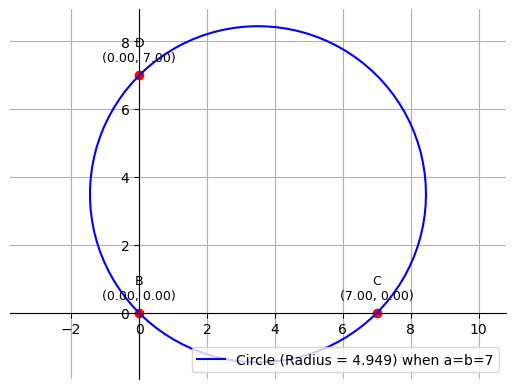
\includegraphics[width=0.7\linewidth]{figs/plot.png}
   \caption{Stem Plot of y\brak{n}}
   \label{stemplot}
\end{figure}
\end{document}  
